\documentclass[12pt,fancy]{cours}
\Chapit{8}{2}
\begin{document}
\maketitre[***]{
L'expression \emph{intelligence artificielle} (IA) a été créée par les américains John McCarty et Marvin Lee Minsky en 1956. Cette époque est marquée par un forte enthousiasme dans le domaine. Les premières IA, comme Eliza, construite au MIT en 1965, étaient capable de dialoguer en anglais en reconstruisant des phrases toutes faites. Pourtant, les intelligences artificielles vraiment performantes ont mis du temps à émerger. À partir des années 80, des outils formels informatiques sont développer pour étudier l'IA : les réseaux de neurone, les algorithmes génératifs, etc. L'IA a réussi à supplanter l'humain dans certains jeux réputés réservés à l'intelligence humaine : citons la machine Deep Blue qui battit G. Kasparov aux échecs en 1997, ou encore la machine AlphoGo qui battit L. Sedol au jeu de go en 2016. 
}{
    \item
}


\section{Introduction}

\begin{definition}\label{def:}
    L'\imp{intelligence artificielle} désigne une machine capable de réaliser des tâches habituellement exécutées par des humains, qui nécessitent des capacités de raisonnement, de mémoire, et d'apprentissage, 
\end{definition}
 En particulier, on souhaite rendre une machine capable d'accéder à certaines connaissances sans avoir été programmée explicitement pour cela, autrement dit capable d'apprendre par elle-même. 
 %  Pour réaliser une machine de ce type, on recourt souvent aux méthodes d'apprentissage automatique.
 Les exemples d'applications de l'IA sont légion. Parmi les grands domaines de l'IA, citons 
 \begin{liste}
    \item la reconnaissance de formes, i.e. de texte, de son (reconnaissance vocale, Alexa, Siri) ou d'images (reconnaissance de visages par la police, analyse d'images médicales) ; 
    \item le traitement du langage naturel, i.e. la reconnaissance vocale, la synthèse vocale (personnes ne pouvant plus parler, génération de chanson), la traduction, les agents conversationnels (chatGBT, chatbots de nombreux sites et applications) ;
    \item les algorithmes de recherche, i.e. google, les filtres de spam ;
    \item la génération de contenu (chatGPT, images artistiques, chansons).
 \end{liste}
  Comme application pluridisciplinaire, citons les voitures autonomes et les robots de compagnie ou d'assistance, qui utilisent le traitement du langage naturel (conversation) et la reconnaissance de formes (mouvement, détection d'obstacle).

  \begin{figure}[H]
    \centering
    \def\sca{4cm}
    % \subfigure[Voitures autonomes]{\label{fig:}
  
    % 
\includegraphics[height=\sca]{self_driving.png}
    % }
    % \subfigure[Reconnaissance vocale]{\label{fig:}
  
    % 
\includegraphics[height=\sca]{Voice_Recognition_Feature_Springwise.jpg}
    % }
    % \subfigure[Agent conversationnel]{\label{fig:}
  
    % 
\includegraphics[height=\sca]{GPT3.jpeg}
    % }
    % \subfigure[Génération d'images artistiques]{\label{fig:}
  
    % 
\includegraphics[height=\sca]{aiart.jpg}
    % }
    
\includegraphics[width=0.9\textwidth]{IA_applications.png}
    \caption{Quelques domaines d'applications de l'intelligence artificielle (IA). (a) Voitures autonomes. (b) Reconnaissance vocale. (c) Agent conversationnel. (d) Génération d'images artistiques.}
    \label{fig:}
  \end{figure}

 \subsection{Apprentissage automatique}
 L'apprentissage automatique (\emph{machine learning}) est un domaine majeur de l'intelligence artificielle.



\begin{definition}
L'\imp{apprentissage automatique} désigne une méthode qui permet à une IA d'apprendre à résoudre un problème sans jamais la programmer explicitement pour résoudre ce problème particulier.
\end{definition}
Une machine \imp{apprend} lorsqu'elle améliore son fonctionnement dans le cadre de la résolution d'un problème : des outils statistiques sont appliqués sur des données et la machine modifie son fonctionnement à partir des résultats de traitement pour améliorer son efficacité. Pour trouver les bons outils statistiques, un modèle est construit à partir des données du problème.
\begin{liste}
    \item L'\imp{algorithme traditionnel} prend en entrée des données et se sert de règles (condition \texttt{if}, boucle \texttt{for}, fonctions mathématiques, etc.) pour produire une réponse en sortie. 
    \item L'\imp{algorithme d'IA}, lors de la phase d'apprentissage, prend en entrée des données (en grande quantité) et éventuellement des réponses (si les données sont déjà étiquetées) et en déduit des règles (de régression, de classification, etc.). 
 \end{liste}
\begin{figure}[H]
    \centering
    \hfill
    % \subfigure[]{\label{fig:}
    % 
\includegraphics[height=0.23\textwidth]{algo_trad.png}
    % }\hfill
    % \subfigure[]{\label{fig:}
    % 
\includegraphics[height=0.23\textwidth]{IA_algo_complet.png}
    % }
    
\includegraphics[width=\textwidth]{algo_comparaison.png}
    % \hfill
    \caption{(a) Principe d'un algorithme traditionnel. L'algorithme prend en entrée des données et se sert de règles (condition \texttt{if}, boucles \texttt{for}, fonctions mathématiques, etc.) pour produire une réponse en sortie. (b) Principe de l'apprentissage d'un algorithme d'intelligence artificielle. Lors de la phase d'apprentissage, l'algorithme prend en entrée des données (en grande quantité) et éventuellement des réponses (si les données sont déjà étiquetées) et en déduit des règles (de régression, de classification, etc.). Lors de la phase d'apprentissage, l'algorithme modifie les règles en affiner la valeur des paramètres de l'algorithme.}
    \label{fig:}
\end{figure}

On caractérise un algorithme d'apprentissage automatique selon sa fonction et la méthode d'apprentissage. Il existe trois techniques principales d'apprentissage automatique. La \imp{fonction} d'un algorithme détermine la nature des règles et l'objectif de l'algorithme. On distingue les algorithmes de
\begin{liste}
    \item \imp{régression} : prédire une nouvelle donnée $y$ à partir d'une donnée $x$ issue d'une variable réelle continue.
    \item \imp{classification} : répartir une nouvelle donnée dans une classe.
    % \item réseaux de neurones artificiels 
\end{liste}
Dans la suite, nous nous intéresserons aux algorithmes de classification. Nous définirons la notion de classification dans la \Sec{classif}.
La \imp{méthode d'apprentissage} détermine la façon dont l'algorithme apprend. On distingue les algorithmes
\begin{liste}
    \item apprentissage \imp{supervisé} : l'algorithme apprend à partir d'un ensemble de données étiquetées (on donne les réponses à l'algorithme). Voir \Sec{supervise}.
    \item apprentissage \imp{non supervisé} : l'algorithme apprend à partir d'un ensemble de données non étiquetées (l'algorithme doit trouver des règles qui fournissent des réponses pertinentes). Voir \Sec{non_supervise}.
\end{liste}
\begin{remarque}
    Il existe d'autres types d'apprentissage comme l'apprentissage par renforcement et l'apprentissage en profondeur.
\end{remarque}


\begin{exemple}{Reconnaissance d'images}
    Un application importante de l'IA est la reconnaissance d'image. On montre ci-dessous une illustration de la phase d'apprentissage automatique d'un algorithme de reconnaissance d'image. 
    \begin{center}
        
\includegraphics[width=\textwidth]{cat_dog.png}
    \end{center}
    % \begin{fig}[cats]
    %     \newcommand{\hei}{2cm}
    %     \centering
    %     \begin{subfig}[cat][0.12][cat]
    %         
\includegraphics[height=\hei]{cat0.jpeg}
    %     \end{subfig}
    %     \begin{subfig}[cat][0.12][cat]
    %         
\includegraphics[height=\hei]{cat1.jpeg}
    %     \end{subfig}
    %     \begin{subfig}[cat][0.12][cat]
    %         
\includegraphics[height=\hei]{cat2.jpeg}
    %     \end{subfig}
    %     \begin{subfig}[dog][0.12][dog]
    %         
\includegraphics[height=\hei]{dog0.jpeg}
    %     \end{subfig}
    %     \begin{subfig}[dog][0.12][dog]
    %         
\includegraphics[height=\hei]{dog1.jpeg}
    %     \end{subfig}
    %     \begin{subfig}[dog][0.12][dog]
    %         
\includegraphics[height=\hei]{dog2.jpeg}
    %     \end{subfig}
    %     % \capt{}
    % \end{fig}
    % \begin{center}
    %   
\includegraphics{cat_analysis.pdf}
    % \end{center}
Une fois l'algorithme entraîné, on exige de l'algorithme qu'il puisse fournir une réponse en sortie lorsqu'on lui donne une image inconnue en entrée, comme ci-dessous.
\begin{center}
    
\includegraphics{cat_analysis_1.pdf}
\end{center}


% Une autre application est la reconnaissance de texte, par exemple la reconnaissance des chiffres de $1$ à $9$. Il s'agit alors de classer l'image dans la bonne catégorie (le bon chiffre).
\begin{quest}
    \item	S'agit-il d'un problème de régression ou de classification ?
    \item S'agit-il d'un apprentissage supervisé ou non supervisé ?
\end{quest}
\end{exemple}
\examplesol{
Algorithme de classification par apprentissage supervisé.
}
% Comme le montre ces exemples, un problème d'apprentissage se ramène souvent à un problème de \imp{classification}. On souhaite une l'apprentissage terminé et la machine fonctionnelle qu'elle puisse attribuer correctement une classe à des données non classés et qu'elle ne connaît pas. L'apprentissage automatique consiste alors à apprendre à la machine comment associer la bonne classe aux données test qu'on lui fournit.


% Il existe plusieurs types d'apprentissage. Nous étudierons les  deux suivants.
% \begin{liste}
% \item L'\imp{apprentissage supervisé}. Les données test sont fournies à la machine avec une classification.
% \item L'\imp{apprentissage non supervisé}. Les données test ne sont pas classées, et c'est à l'IA de déterminer les classes à partir de la structure des données.
% \end{liste}


\subsection{Algorithmes de classement}
\label{sec:classif}

Dans le cadre du cours, nous étudierons des problèmes de classement, plus spécifiquement des problèmes de classement exclusif, ou chaque donnée ne peut exister que dans un seul groupe. 
Considérons un ensemble de données $E$ (images, sons, textes...) de $N$ éléments.

\begin{definition}[Classification]
On appelle \imp{classification} des données une partition de $E$, c'est-à-dire une famille de sous-ensembles $E_i \subset E, i=1,...,n$ :
\begin{liste}
\item dont la réunion décrit l'ensemble entier (tous les éléments sont classés) : $\displaystyle\cup_{i} E_i = E$ ;
\item disjoints (un élément n'appartient qu'à une seule classe) : $E_i \cap E_j = \varnothing$ si $i\neq j$.
\end{liste}
\end{definition}

On peut représenter un ensemble d'apprentissage $E$ de $N$ données en \texttt{python} par une liste \texttt{[y1,y2,...,yN]}.
Un méthode efficace pour définir une partition sous \texttt{python} est d'utiliser un dictionnaire.

\begin{prop}\label{prop:}
On représente une classification $(E_i)_{i=1,...n}$ sous \texttt{python} par un \imp{dictionnaire} 
\begin{center}
\texttt{p=\{y1:c1, y2:c2, ..., yN:cN\}}
\end{center}
où les $y_j$ sont les éléments de $E=\cup_{i} E_i $ et $c_j$ désigne la classe à laquelle appartient $y_j$ (l'un des $E_i$).
\end{prop}
\begin{remarque}
    La recherche de la classe d'un élément $x$ de $E$ exige alors une complexité constante $O(1)$, grâce à la structure de dictionnaire.
    En définissant la partition comme une liste \texttt{p=[[y1,c1], [y2,c2], ..., [yN,cN]]}, on obtiendrait une complexité linéaire en $O(N)$.
\end{remarque}

\begin{exemple}{Reconnaissance d'images}
    Quelle est la classification des images de l'exemple précédent ? La définir sous \texttt{python}.
\end{exemple}
\examplesol{
    La classification est $E=\text{chats} \cup \text{chiens}$ où chats$\,=\{a,b,c\}$ contient les 3 premières images et chiens$\,=\{d,e,f\}$ les 3 suivantes. Sous python, on peut définir l'ensemble de données $E$ sous forme d'une liste de caractères désignant chaque image,
    \eqbox{
        \texttt{E = [`a', `b', `c', `d', `e', `f']}.
    }
    Les classes sont les chaînes de caractères \texttt{`chat'} et \texttt{`chien'}.
    La classification est définie par le dictionnaire
    \eqbox{
        \texttt{p = \{`a':`chat', `b':`chat', `c':`chat',  `d':`chien', `e':`chien', `f':`chien'\}}.
    }
}


\begin{exemple}{Recherche d'articles de presse}
    \label{ex:articles}
    On souhaite proposer un algorithme de recherche d'articles de presse suivant leur sujet. On considère $5$ particles de presse appartenant à $2$ classes : les sujets « culture » et « science ». Les articles sont modélisés par un point $y=(c,s)$ du plan où $c$ représente la fréquence du mot « culture » et $s$ la fréquence du mot « science » dans le corps de l'article.

    \begin{center}
        \begin{tabular}{|c|c|c|c|c|c|}
            \hline
            Articles & Article 1 & Article 2 & Article 3 & Article 4 & Article 5 \\
            \hline
            c & 0.8 & 0.2 & 0.6 & 0.4 & 0.9 \\
            \hline
            s & 0.5 & 0.9 & 0.3 & 0.7 & 0.2 \\
            \hline
            Sujet & Culture & Science & Culture & Science & Culture \\
            \hline
        \end{tabular}
    \end{center}

    \begin{quest}
        \item Définir formellement puis en \texttt{python} l'ensemble d'apprentissage $E$.
        \item Définir formellement puis en \texttt{python} la classification $(E_i)_{i=1,...n}$ associée.
    \end{quest}
    
    % On dispose d'un ensemble de données $E$ contenant $N=1000$ articles de presse. On souhaite classer ces articles en $n=5$ catégories : \{politique, économie, sport, culture, faits divers\}. On peut définir la classification sous python par le dictionnaire
% On considère un ensemble d'apprentissage $E$ contenant $N=250$ points du plan de coordonnées $P=(x,y)$, voir \Fig{xy}. Ces données sont réparties en deux classes selon la couleur du point : \{rouge, bleu\}. On peut coder l’ensemble $E$ sous python avec une liste,
% $$
% \texttt{E = [(0.8,0.5), (0.2,0.9), (0.6,0.3), (0.4,0.7), (0.9,0.2)]}.
% $$
% On peut ensuite définir la classification associé par les chaînes de caractère \texttt{`bleu'} et
%  \texttt{`rouge'}.
%  $$
%  \texttt{p = \{(x1,y1):`bleu', (x2,y2):`rouge', ..., (xN,yN):`bleu'\} }.
%  $$

% %%%%%%%%%%%%%%%%%%%%%%%%%
% \begin{fig}[xy]
% \centering
% 
\includegraphics[width=0.3\textwidth]{xy_couleur.png}
% \capt{Exemple de série de données $E$ constituée de points du plan $P=(x,y)$, de couleur rouge ou bleue.}
% % \label{fig:xy}
% \end{fig}
% %%%%%%%%%%%%%

\end{exemple}
\examplesol{
    \begin{quest}
        \item  On peut coder l’ensemble $E$ sous python avec une liste,
        \eqbox{
            \texttt{E = [(0.8,0.5), (0.2,0.9), (0.6,0.3), (0.4,0.7), (0.9,0.2)]}.
        }
        \item On peut ensuite définir la classification mathématiquement par $E = \text{culture } \cup \text{ science}$ où culture$\,=\{(0.8,0.5), (0.6,0.3), (0.9,0.2)\}$  et science$\,=\{(0.2,0.9), (0.4,0.7)\}$. On peut définir la classification sous python par le dictionnaire 
        % \eqbox{
            \begin{center}
                
                \texttt{p = \{(0.8,0.5):`culture', (0.2,0.9):`science', (0.6,0.3):`culture',} 
                \texttt{
                    (0.4,0.7):`science', (0.9,0.2):`culture'\} }.
                \end{center}
        % }
    \end{quest}
}

\section{Apprentissage supervisé}

Nous nous intéressons ici à l'apprentissage supervisé des algorithmes de classement. Le développement d'un algorithme d'IA comprend deux phases :
\begin{liste}
    \item l'apprentissage (\Sec{kvoisins});
    \item le test (\Sec{test});
\end{liste} 
L'algorithme de classement standard pour réaliser un apprentissage supervisé  est l'algorithme des $k$ plus proches voisins.


\subsection{Algorithme des $k$ plus proches voisins}
\label{sec:kvoisins}

\parag{Notion de distance} Considérons un ensemble de données $E$ contenant $N$ éléments, et une classification de $E$, noté $(E_i)_{i=1,...n}$. Les donnés sont donc réparties en $n$ classes bien déterminées. Cet ensemble $E$ est appelé \imp{ensemble d'apprentissage}.

Soit une donnée $x$ qui n'appartient pas à $E$. On souhaite classer $x$ selon la classification $(E_i)_{i=1,...n}$ c'est-à-dire trouver la classe $i$ dont les éléments sont les \guill{plus proches} de $x$. Pour cela, il faut définir une notion de distance, qui dépend de la nature des données de $E$ et du problème.

\begin{definition}[Distance]\label{def:dist}
    Une \imp{distance} est une fonction $d(x,y)$ de deux données $x$ et $y$ de l'ensemble d'apprentissage $E$.
\end{definition}
Lorsque les données sont des nombres entiers ou réels, il est naturel d'utiliser la distance \imp{euclidienne}. Pour des points $x=(x_1,x_2)$ et $y=(y_1,y_2)$ du plan, par exemple, la distance euclidienne est définie par 
    % \begin{equation}
    \eqbox[d_euclid]{
        d(x,y) = \sqrt{(x_1-y_1)^2 + (x_2 - y_2)^2}.
        }
    % \end{equation}
\begin{exemple}{Exemples de distance}
\begin{quest}
    \item Pour des points du plan $x=(x_1,x_2)$ et $y=(y_1,y_2)$ définis sur une grille, on peut utiliser la distance de Manhattan, définie par 
    \begin{equation}
        d_{\rm M}(x,y) = |x_1-y_1| + |x_2 - y_2|.
    \end{equation} 
    Justifier le nom donner à cette distance. Que vaut $d_{\rm M}((1,2),(3,4))$ ?
    \item On suppose que les données de $E$ sont des images en niveau de gris. En supposant les couleurs codées sur $8$ bits, dans quel ensemble mathématique appartient le niveau de gris $G(x)$ d'un pixel $x$ ? Définir une distance $d_{\rm g}$ qui compare les niveaux de gris des mêmes pixels $x$ et $y$ pris de deux images différentes. 
    \item On suppose que les données de $E$ sont des chaînes de caractères. On définit la distance de Hamming $d_{\rm H}(x,y)$ comme le nombre de caractères à modifier pour passer de la chaîne $x$ à la chaîne $y$. Par exemple, la distance de Hamming entre les mots « ramer » et « cases » vaut $3$. Que vaut la distance de Hamming pour : les mots « chanter » et « chat » ; les nombres binaires 0110 et 1110 ? 
    %  la distance peut être la proximité de forme. Par exemple, les caractères $b$ et $p$ peuvent être considérés proches car tous deux présentent une boucle.
    \end{quest}    
\end{exemple}
\examplesol{
\begin{quest}
    \item  $G(x) \in [0,255]$. La différence de niveau de gris entre deux pixels $x$ et $y$ peut s'évaluer par la distance
    $d_{\rm gris}(x,y) = |G(x)-G(y)|$.
\end{quest}
}


% Dans tous les cas, on suppose que la proximité entre deux données $x$ et $y$ peut se quantifier à l'aide d'une fonction distance $d(x,y)$ défini sur un espace à $D$ dimensions.

\parag{Principe de l’algorithme} L'algorithme des $k$ plus proches voisins est paramétré par un entier $k<N$. On suppose avoir défini une distance $d$ sur l'ensemble d'apprentissage. Soit un élément $x$ n'appartenant pas à $E$ à classer (carré vert sur la \Fig{knna}). On commence par calculer les distances $d(x,y)$ entre $x$ et chaque élément $y$ de $E$ (\Fig{knnb}). On détermine ensuite les $k$ plus proches voisins (\Fig{knnc}). Puis on détermine la classe majoritaire des voisins (\Fig{knnd}). 

\begin{figure}[H]
    \centering
    
\includegraphics[width=\textwidth]{algo_k_voisins.png}
%     \subfigure[Nouvelle donnée]{\label{fig:knna}
%     
\includegraphics{principe_knn_0.pdf}
%     }
%     \subfigure[Calcul de distance]{\label{fig:knnb}
%     
\includegraphics{principe_knn_1.pdf}
%     }
%     \subfigure[Estimation des voisins]{\label{fig:knnc}
%     
\includegraphics{principe_knn_2.pdf}
%     }
%     \subfigure[Attribution classe majoritaire]{\label{fig:knnd}
% 
\includegraphics{principe_knn_3.pdf}
% }
    \caption{Principe de l'algorithme des $k$ plus proches voisins. (a) On considère un ensemble d'apprentissage $E$ contenant $N$ éléments. (b) On souhaite classer un nouvel élément $x$ n'appartenant pas à $E$. (c) On détermine les $k$ plus proches voisins de $x$ dans $E$. On associe à $x$ la classe majoritaire des voisins. (d) On associe à $x$ la classe majoritaire des voisins.}
    \label{fig:}
\end{figure}

\begin{definition}[Algorithme des $k$ plus proches voisins]
\begin{enumerate}
\item On trie l'ensemble $E$ suivant l'ordre croissant des distances à $x$, c'est-à-dire la valeur de $d(x,y)$ avec $y\in E$. On obtient une liste à $N$ éléments {\rm{tri}}$(E,x,d)$.
\item On choisit les $k$ plus proches voisins, c'est-à-dire les $k$ premiers éléments de {\rm{tri}}$(E,x,d)$. On obtient la liste {\rm{voisins}}$(E,x,d,k)$.
\item On détermine la classe dominante de {\rm{voisins}}$(E,x,d,k)$, notée {\rm classemaj}$(E, x, d, k, p)$ c'est-à-dire qu'on détermine la classe $i$ telle que l'intersection $E_j\, \cap $ {\rm{voisins}}$(E,x,d,k)$ contienne le maximum d'éléments pour $j=i$. On associe ainsi la classe $i$ au nouvel élément $x$.
\end{enumerate}
\end{definition}
\noindent
Nous implémenterons  en \texttt{python}  les fonctions {\rm{tri}}$(E,x,d)$, {\rm{voisins}}$(E,x,d,k)$ et {\rm classemaj}$(E, x, d, k, p)$ en TD. Pour l'instant, nous allons appliquer l'algorithme des $k$ plus proches voisins sur un exemple simple sans se soucier de l'implémentation des fonctions.

\begin{exemple}{Recherche d'articles de presse}
    Reprenons l'exemple de recherche d'articles de presse, Ex.~\ref{ex:articles}. Un auteur publie un nouvel article sur le site internet du magazine (Article 6) dont la fréquence du mot « culture » est $c=0.6$ et la fréquence du mot « science » est $s=0.5$. On souhaite classer cette nouvelle donnée $x=(0.6,0.5)$ dans l'une des deux classes « culture » ou « science » en s'aidant de l'ensemble d'apprentissage $E$ précédent. On utilise la distance euclidienne.
    %  $d(x,y) = \sqrt{(x_1-y_1)^2 + (x_2 - y_2)^2}$.

    % \begin{center}
    %     \begin{tabular}{|c|c|c|c|c|c|}
    %         \hline
    %         Articles & Article 1 & Article 2 & Article 3 & Article 4 & Article 5 \\
    %         \hline
    %         c & 0.8 & 0.2 & 0.6 & 0.4 & 0.9 \\
    %         \hline
    %         s & 0.5 & 0.9 & 0.3 & 0.7 & 0.2 \\
    %         \hline
    %         Sujet & Culture & Science & Culture & Science & Culture \\
    %         \hline
    %     \end{tabular}
    % \end{center}

    \begin{quest}
        \item Rappeler la définition de la distance euclidienne dans ce contexte.
        \item Déterminer la liste triée des éléments de $E$ suivant l'ordre croissant des distances à $x$. Représenter l'ensemble des données $E$ et $x$ sur un graphique.
        \item Déterminer les $k=3$ plus proches voisins de $x$ dans $E$. Représenter les $k$ plus proches voisins sur le graphique. Pourquoi est-il préférable de choisir un nombre impair $k$ de voisins ?
        \item Déterminer la classe majoritaire des voisins. En déduire la classe de $x$.
    \end{quest}

    \examplesol{
        \begin{quest}
            \item La distance euclidienne entre deux points $x=(c_1,s_1)$ et $y=(c_2,s_2)$ du plan est donnée par
            $$
            d(x,y) = \sqrt{(c_1-c_2)^2 + (s_1 - s_2)^2}.
            $$
            \item On calcule les distances entre $x$ et chaque élément de $E$. On obtient la liste triée suivante
            \eqbox{
                \text{{\rm{tri}}}(
                    E,x,d) = \left[
                        (0.4,0.7) ,
                        (0.7,0.5),
                        (0.6,0.3) ,
                        (0.8,0.5) ,
                        (0.2,0.9)
                        \right].
            }
            On représente les données sur le graphique ci-dessous.
            \begin{center}
                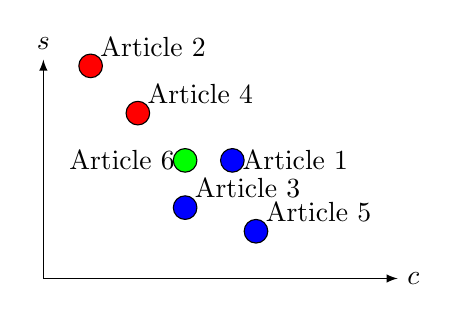
\begin{tikzpicture}[scale=3]
                    \draw[->,>=latex] (0,0) -- (0,1.5/1.618) node[above] {$s$};
                    \draw[->,>=latex] (0,0) -- (1.5,0) node[right] {$c$};
                    \draw[fill=blue] (0.8,0.5) circle (0.05) node[right=0.2] {Article 1};
                    \draw[fill=red] (0.2,0.9) circle (0.05) node[above right] {Article 2};
                    \draw[fill=blue] (0.6,0.3) circle (0.05) node[above right] {Article 3};
                    \draw[fill=red] (0.4,0.7) circle (0.05) node[above right] {Article 4};
                    \draw[fill=blue] (0.9,0.2) circle (0.05) node[above right] {Article 5};
                    \draw[fill=green] (0.6,0.5) circle (0.05) node[left=0.2] {Article 6};
                \end{tikzpicture}
            \end{center}
            \item Les $k=3$ plus proches voisins de $x$ sont les trois premiers éléments de la liste triée. On obtient
            \eqbox{
                \text{{\rm{voisins}}}(
                    E,x,d,3) = \left[
                        (0.7,0.5),
                        (0.6,0.3),
                        (0.8,0.5)\right].
            }
            On représente les $k$ plus proches voisins sur le graphique ci-dessous.
            \begin{center}
                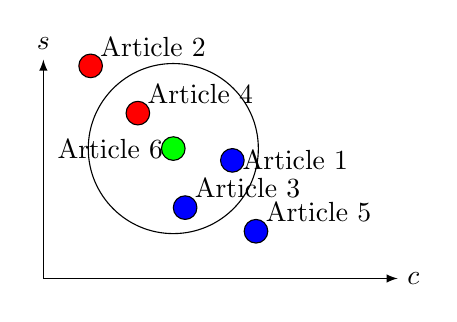
\begin{tikzpicture}[scale=3]
                    \draw[->,>=latex] (0,0) -- (0,1.5/1.618) node[above] {$s$};
                    \draw[->,>=latex] (0,0) -- (1.5,0) node[right] {$c$};
                    \draw[fill=blue] (0.8,0.5) circle (0.05) node[right=0.2] {Article 1};
                    \draw[fill=red] (0.2,0.9) circle (0.05) node[above right] {Article 2};
                    \draw[fill=blue] (0.6,0.3) circle (0.05) node[above right] {Article 3};
                    \draw[fill=red] (0.4,0.7) circle (0.05) node[above right] {Article 4};
                    \draw[fill=blue] (0.9,0.2) circle (0.05) node[above right] {Article 5};
                    \draw[fill=green] (0.55,0.55) circle (0.05) node[left=0.2] {Article 6};
                    \draw (0.55,0.55) circle (0.36);
                \end{tikzpicture}
            \end{center}
            Il est préférable de choisir un nombre impair de voisins pour éviter les situations d'égalité.
            \item La classe majoritaire des voisins est la classe « culture ». On en déduit que l'article 6 est un article de culture.
            \eqbox{
                \text{\rm{classe}}(E,x,d,3) = \text{culture}.
            }
        \end{quest}
    }
\end{exemple}


% L'algorithme des $k$ plus proches voisins peut s'implémenter de la façon suivante.
% \begin{enumerate}
% \item On trie l'ensemble $E$ suivant l'ordre croissant des distances à $x$, c'est-à-dire la valeur de $d(x,y)$ avec $y\in E$.
% \inputminted{python}{./code/tri_xy.py}
% \item On choisit les $k$ plus proches voisins, c'est-à-dire les $k$ premiers éléments de {\rm{tri}}$(E,x,d)$.
% \inputminted{python}{./code/voisins_xy.py}
% \item On détermine la classe dominante de {\rm{voisins}}$(E,x,d,k)$, c'est-à-dire qu'on détermine la classe $i$ telle que l'intersection $E_j\, \cap $ {\rm{voisins}}$(E,x,d,k)$ contienne le maximum d'éléments pour $j=i$. Pour cela on se donne une partition $p$ sous forme de dictionnaire.
% \inputminted{python}{./code/classe_xy.py}
% \end{enumerate}

\parag{Critique de l’algorithme} Cet algorithme possède certains avantages et inconvénients.
% \imp{Avantages}.
\oneitem[.]{Avantages}
\begin{enumerate}
    \item L’algorithme est \emph{simple}, et facile à implémenter, comme nous le verrons en TD.
    \item L'algorithme nécessite \emph{peu de paramètres} : la distance $d$ et le nombre de voisins $k$.
\end{enumerate}

\oneitem[.]{Inconvénients}
\begin{enumerate}
    \item L'algorithme est \emph{paresseux} : au lieu de subir une longue phase d'entraînement pour optimiser les paramètres de l'algorithme, l'algorithme sollicite l'ensemble d'apprentissage entier pour réaliser une prédiction. Solliciter une quantité aussi importante de données à chaque fois peut être coûteux en mémoire, en temps et en argent.
    \item L'algorithme fonctionne mal avec des données de \emph{grande dimension} (grand nombre de coordonnées).
    \item L'algorithme est \emph{sensible} au choix du nombre de voisins $k$. Si l'on avait choisi $k=1$, on aurait trouvé dans l'exemple précédent que le plus proche voisin du nouvel article est ($0.7,0.5$), qui est un article de science. L'algorithme aurait donc classé l'article 6 comme un article de science.
    \begin{center}
        
\includegraphics{critere_classemaj}
        % \begin{tikzpicture}[scale=3]
        %     \draw[->,>=latex] (0,0) -- (0,1.5/1.618) node[above] {$s$};
        %     \draw[->,>=latex] (0,0) -- (1.5,0) node[right] {$c$};
        %     \draw[fill=blue] (0.8,0.5) circle (0.05) node[right=0.2] {Article 1};
        %     \draw[fill=red] (0.2,0.9) circle (0.05) node[above right] {Article 2};
        %     \draw[fill=blue] (0.6,0.3) circle (0.05) node[above right] {Article 3};
        %     \draw[fill=red] (0.4,0.7) circle (0.05) node[above right] {Article 4};
        %     \draw[fill=blue] (0.9,0.2) circle (0.05) node[above right] {Article 5};
        %     \draw[fill=green] (0.55,0.55) circle (0.05) node[left=0.2] {Article 6};
        %     \draw (0.55,0.55) circle (0.25);
        % \end{tikzpicture}
    \end{center}
    \item Le choix de la \emph{classe majoritaire} n'est pas forcément le meilleur critère.  En effet, ce choix ne prend pas en compte la distribution des classes des voisins. Comme le montre l'exemple ci-dessus, la classe majoritaire ne correspond pas forcément à la classe du plus proche voisin.  Pour améliorer la détermination de la classe, on peut par exemple pondérer les classes par la distance entre les voisins et le point $x$ à classer.
    % \item L'algorithme est sensible au choix de la distance $d$. En effet, le choix de la distance dépend de la nature des données et du problème. Il n'existe pas de distance universelle.
\end{enumerate}
% plusieurs limites.
% \begin{liste}
% \item Détermination de la classe.

% Classer $x$ dans la classe majoritaire des voisins n’est pas forcément le meilleur choix. Par exemple, on pourrait travailler sur des points  colorés selon plusieurs nuances de bleu et de rouge. La classe majoritaire des voisins de $x$ peut très bien être rouge, alors que la plupart des voisins sont bleus.
% \begin{center}
% 
\includegraphics[scale=1]{histo.pdf}
% \end{center}

% % \end{liste}

\subsection{Matrice de confusion}
\label{sec:test}

\parag{Définitions et exemples}
L’algorithme des $k$ plus proches voisins permet d’effectuer des prédictions pendant la phase d'apprentissage finie. Afin d'améliorer ou de contrôler le bon fonctionnement de l'IA, il faut mesurer la qualité de ces prédictions. Pour cela, on introduit la notion de matrice de confusion.

\begin{exemple}{Test médical}
Considérons un test médical destiné à déterminer la présence ou non d’une infection chez un groupe de $100$ patients.
L’efficacité du test n’est pas parfaite. On suppose que $90$ prédictions du test sont corrects, tandis que $10$ prédictions sont fausses.
\begin{liste}
    \item Parmi les tests corrects,  $20$ sont de vrai positifs, et $70$ des vrais négatifs.
    \item Parmi les tests incorrects, $8$ sont de faux négatifs, et $2$ des faux positifs.
\end{liste}
Représenter les données dans le tableau suivant.

\begin{center}
\begin{tabular}{llll}
& & \textbf{Classe prédite} & \\
& & Infecté & Sain \\
\textbf{Classe réelle} & Infecté & ... & ...\\
 & Sain & ... & ... \\
\end{tabular}
\end{center}
\end{exemple}
\examplesol{
\begin{center}
\begin{tabular}{llll}
& & \textbf{Classe prédite} & \\
& & Infecté & Sain \\
\textbf{Classe réelle} & Infecté & $20$ (vrai positif) & $8$ (faux négatif)\\
& Sain & $2$ (faux positif) & $70$ (vrai négatif) \\
\end{tabular}
\end{center}
}

On peut généraliser cet exemple à des données issues de prédictions d’une IA. Considérons un ensemble données, appelé ensemble de test $T$. Notons $(T_i)_{i=1,...n}$ la classification de $T$. Les données test sont donc réparties en $n$ classes bien déterminées. On applique un algorithme d’apprentissage, qui à chaque donnée $x\in T$ associe une classe $T_j$, pour un certain $j=1,...n$. On appelle $T_i$ la classe réelle de $x$ et $T_j$ la classe prédite de $x$.
%  On peut alors définir la matrice de confusion.
\begin{definition}[Matrice de confusion]
On appelle \imp{matrice de confusion} la matrice $M$ de taille $n\times n$ (avec $n$ le nombre de classes) dont
\begin{liste}
\item chaque ligne $i$ correspond à une classe réelle $T_i$ ;
\item chaque colonne $j$ correspond à une classe prédite $T_j$ ;
\item chaque élément $M_{ij}$ donne le nombre de données de classe réelle $T_i$ et de classe prédite $T_j$.
\end{liste}
\end{definition}
%Une matrice de confusion permet d’estimer la qualité des prédictions.
Dans une matrice de confusion, chaque élément de la \imp{diagonale} correspond à des points correctement classés. Chaque élément \imp{hors diagonal} correspond à des points mal classés. À partir de la matrice de confusion, on peut définir plusieurs grandeurs pour quantifier la qualité des prédictions.

% \begin{figure}[H]
%     \centering
%     
\includegraphics{matrice_confu.pdf}
%     \caption{Matrice de confusion. Le nombre de prédictions correctes est $N_c$, le nombre de prédictions incorrectes est $N_i$.}
%     \label{fig:}
% \end{figure}

\begin{liste}
\item Le \imp{taux d’erreur} TE est le nombre de prédictions incorrectes $N_i$ sur le nombre total de prédictions~$N$,
\eqbox{
    \text{TE } = \frac{N_i}{N}.
}
On vise un taux d’erreur le plus proche possible de $0$.
\item La \imp{précision} est le nombre de prédictions correctes $N_c$ sur le nombre total de prédictions~$N$,
\eqbox{
    \text{P} = \frac{N_c}{N} = 1 -\text{TE}.
}
\end{liste}
\begin{remarque}
    
    Dans le cas où il n’existe que deux classes, \guill{positif} et \guill{négatif}, on définit aussi les grandeurs suivantes.
    \begin{liste}
\item La \imp{sensibilité} est le nombre de positifs corrects $p_c$  sur le nombre total de positifs~$p$,
\begin{equation}
    s = \frac{p_c}{p}.
\end{equation}
Le taux de faux positifs vaut alors TFP $= 1-s$.
\item La \imp{spécificité} est le nombre de négatifs corrects $n_c$  sur le nombre total de négatifs $n$,
\begin{equation}
    \overline{s} = \frac{n_c}{n}.
\end{equation}

\end{liste}
\end{remarque}


\begin{exemple}{Caractéristiques d’un test médical}
Considérons le test médical suivant.
\begin{center}
\begin{tabular}{llll}
& & \textbf{Classe prédite} & \\
& & Infecté & Sain \\
\textbf{Classe réelle} & Infecté & $20$ (vrai positif) & $8$ (faux négatif)\\
 & Sain & $2$ (faux positif) & $70$ (vrai négatif) \\
\end{tabular}
\end{center}
\begin{quest}
    \item Que vaut le nombre de données $N$ ? Que vaut le nombre de données correctes $N_c$ ? Que vaut le nombre de données incorrectes $N_i$ ?
    \item Calculer la précision P et le taux d’erreur TE.
    \item Calculer le nombre de négatifs $n$ et le nombre de positifs $p$. En déduire la sensibilité $s$ et la spécificité $\overline{s}$.
    \item On définit le taux de négatifs ${\rm TN} = \frac{n}{N}$. Trouver une relation littérale entre $s$, $P$ et ${\rm TN}$.
\end{quest}
\end{exemple}
\examplesol{
    \begin{quest}
        \item Le nombre de données test vaut $N=100$, pour $N_i=10$ données incorrectes et $N_c = 90$ données correctes.
        \item Le taux d’erreur vaut donc TE $=10/100=\num{0.1}$, pour une précision P $=90/100=\num{0.9}$.
        \item Le nombre de prédictions positives correctes vaut $p_c=20$, tandis que le nombre total de prédictions positives vaut $p=22$. La sensibilité vaut donc $s=20/20=\num{0.91}$. Le nombre de prédictions négatives correctes vaut $\overline{p}_c=70$, tandis que le nombre total de prédictions négatives vaut $\overline{p}=78$. La spécificité vaut donc $\overline{s}=70/78=\num{0.90}$. 
        \item On a également les relations $p + n = N$ et $p_c + n_c = N_c$. Ainsi, $\overline{s} = -\frac{p_c}{n} + \frac{N_c}{n} = -s \frac{p}{n} + P \frac{N}{n} = -s(\frac{N}{n}-1) + P \frac{N}{n} = (P-s)\frac{N}{n}+s$ où $\frac{n}{N}=TN$ représente le taux de négatifs. Ainsi, 
        \eqbox{
            \overline{s} = s+\frac{P-s}{TN}.
        }
    \end{quest}
}
%Si l’on normalise la matrice de confusion par le nombre $N$ d’éléments, on obtient alors la matrice suivante
%\begin{center}
%\begin{tabular}{llll}
%& & \textbf{Classe prédite} & \\
%& & Infecté & Sain \\
%\textbf{Classe réelle} & Infecté & $20$ (vrai positif) & $8$ (faux négatif)\\
% & Sain & $2$ (faux positif) & $70$ (vrai négatif) \\
%\end{tabular}
%\end{center}

\parag{Implémentation}

La détermination de la matrice de confusion peut s'implémenter de la façon suivante. On peut représenter la matrice de confusion par une liste de liste. La fonction prend en argument : l’ensemble d’apprentissage $E$, l’ensemble test $T$, la distance $d$, le nombre de plus proches voisins $k$, et la partition (classification) $p$. Pour simplifier, les classes sont associées à des entiers $i,j = 0,...,n-1$.
\inputminted{python}{./code/matrice_confus.py}
Connaissant la matrice de confusion, on peut ensuite calculer le taux d’erreur ou la précision, comme dans l’exemple ci-dessous. La fonction \texttt{precision} prend en argument la matrice de confusion $M$ et le nombre de prédictions $N$, et renvoie la précision $P$.
\inputminted{python}{./code/precision.py}

\begin{exemple}{Implémentation de test de qualité des prédictions}
    Pour chacune des fonctions ce-dessous, on précisera les spécifications de cette fonction et on la commentera. Tester cette fonction sur un exemple.
    \begin{quest}
        \item Définir en \texttt{python} une fonction \texttt{erreur} qui prend comme seul argument  la matrice $M$ \emph{de taille quelconque} et qui calcule le taux d'erreurs du test. 
        \item Définir en \texttt{python} une fonction \texttt{sensibilite} qui prend comme seul argument  la matrice $M$ de taille $2$ par $2$ et qui calcule la sensibilité du test. 
        \item Définir en \texttt{python} une fonction \texttt{specificite}  qui prend comme seul argument  la matrice $M$ de taille $2$ par $2$  et qui calcule la spécificité du test. 
        \item Définir en \texttt{python} une fonction \texttt{prevalence} qui prend comme seul argument la matrice $M$ de taille $2$ par $2$  et qui calcule la prévalence du test, c’est-à-dire le nombre de patients infectées sur le nombre total de patients.
    \end{quest}
\end{exemple}
\examplesol{
    {\rm 
    \inputminted{python}{\pathtoexos/Info/Scripts/sens.py}
    }
}

\section{Apprentissage non supervisé}

L'apprentissage \imp{non supervisé} utilise des
algorithmes d'apprentissage automatique pour analyser et regrouper des jeux de données
non étiquetés. Nous appliquerons ces algorithmes dans des problèmes de classement, plus spécifiquement au classement exclusif, ou chaque donnée ne peut exister que dans un seul groupe.  Dans cette partie, nous nous intéresserons uniquement à la phase d'apprentissage de l'algorithme (la phase de test est similaire à celle de l'apprentissage supervisé avec la matrice de confusion).

\subsection{Algorithme des $k$ moyennes}

\parag{Principe de l’algorithme} Dans un apprentissage non supervisé, c’est à la machine de trouver des éléments de similarités dans les données et d’en déduire les classes. La partition $p$ n’est donc pas donnée ! On impose par contre à la machine le nombre $k$ de classes à définir.

Pour partitionner les données, on initialise chaque groupe $i$ par une donnée centrale $c_{i}$ pour $i=1,...,k$. Ces centres peuvent par exemple être choisis aléatoirement dans l’ensemble d’apprentissage $E$. On définit ensuite la partition initiale en classant les points de $E$ selon leur proximité avec les centres $c_{i}$. La proximité entre les données se mesure, comme pour l’apprentissage supervisé, avec une distance~$d$.
À chaque itération, on affine le partition en calculant pour chaque groupe les barycentres des groupes, qui servent de nouveaux centres pour le partitionnement.


\begin{definition}[Algorithme des $k$ moyennes]
    Soit un ensemble d'apprentissage $E$, deux entiers $k\geq1$ et $n_i\geq 1$, et $d$ une distance.
\begin{enumerate}
\item Initialiser aléatoirement les centres $c_{i}$ parmi les éléments de $E$ pour $i=1,...,k$.
%  fonction \texttt{centres(E,k)}.
\item À chaque itération$j=1,...,n_i$, effectuer :
\begin{liste}
\item partitionnement de $E$ autour des centres $c_i$ selon la distance $d$ ;
%  : fonction \texttt{partition(E, k, centres, d)}
\item ré-évaluation des centres $c_i$ comme barycentre du groupe $E_i$.
%  : \texttt{bary(points)}
\end{liste}
\end{enumerate}
\end{definition}

\begin{remarque}
Pour pouvoir définir un barycentre, il faut que $E$ provienne d’un ensemble dont la structure est celle d’un espace affine. En particulier, il doit exister une opération $+$ dans $E$, ce qui permet d’additionner des points, et une opération de multiplication par un scalaire.
\end{remarque}


\begin{figure}[H]
    \centering
    \subfigure[Ensemble d'apprentissage]{\label{fig:knna}
    
\includegraphics{principe_kmoy_0.pdf}
    }
    \subfigure[Choix aléatoire de centres]{\label{fig:knnb}
    
\includegraphics{principe_kmoy_00.pdf}
    }
    \subfigure[Partitionnement suivant la distance]{\label{fig:knnc}
    
\includegraphics{principe_kmoy_1.pdf}
    }
    \subfigure[Évaluation des centres comme barycentres]{\label{fig:knnd}

\includegraphics{principe_kmoy_3.pdf}
}
    \caption{Principe de l'algorithme des $k$ moyennes. (a) On considère un ensemble d'apprentissage $E$ contenant $N$ éléments. (b) On choisit aléatoirement $k$ centres parmi les données de $E$. (c) On partitionne $E$ suivant la distance aux centres. (d) On ré-évalue les centres comme barycentre de chaque classe. On réitère ensuite le processus.}
    \label{fig:}
\end{figure}

 
\parag{Programmation} On peut programmer chaque étape de la façon suivante.

\begin{enumerate}
    \item 
Commençons par initialiser les centres à partir d’un ensemble d’apprentissage $E$ et d’un nombre de classes $k$. Pour cela, on peut utiliser la fonction \texttt{sample} de la bibliothèque \texttt{random}, avec la commande \texttt{sample(E, k)}, qui renvoie une liste de $k$ éléments distincts choisis aléatoirement dans $E$.

\inputminted{python}{./code/centres.py}
\item
    On définit maintenant une fonction \texttt{partition} qui partitionne $E$ autour des centres $c_i$ pour $i=0,...,k-1$, représentés par une liste \texttt{centres}, selon la distance $d$. On assimile une classe à l’indice $i$ du centre $c_i$, élément de la liste \texttt{centres = [c0,c1,...,ck-1]}. On peut pour cela utiliser la fonction 
    \begin{minted}{python}
    min(centres, key = lambda y:d(x,y))
    \end{minted}
    que renvoie le centre $c$ dont la distance $d(x,c)$ est minimale pour la donnée $x$. Cette ligne est équivalente au code :
    \begin{minted}{python}
    c    = centres[0]
    dist = d(x,c)
    for y in centres[1:]:
        if d(x,y) < dist:
            c    = y
            dist = d(x,y)
    return c
    \end{minted}
    On peut ensuite coder la fonction \texttt{partition} de la façon suivante.
    %Pour cela, on utilise la fonction \texttt{tri(E, x, d)} définie plus haut qui trie les éléments de $E$ par ordre croissant de distance à $x$.
    \inputminted{python}{./code/partition.py}
    
     Une fois une partition définie, nous devons ré-évaluer les centres comme barycentre des classes $E_i$. On rappelle que le barycentre $B$ d'un ensemble de points $\{M_1,...,M_N\}$ est donné par 
     \begin{equation}
        \Vec{OB} = \frac{1}{n}\sum_{j = 1}^N \Vec{OM_j}.
    \end{equation}
     où $O$ est l'origine. Si les points appartiennent au plan et sont de coordonnées $M_j=(x_{1j},x_{2j})$, on peut projeter sur les axes de sorte que $B = (b_1,b_2)$ avec
     
        \begin{equation}
            b_1 = \frac{1}{N}\sum_{j = 1}^N x_{1j} \quad \text{et} \quad b_2 = \frac{1}{N}\sum_{j = 1}^n x_{2j}.
        \end{equation}
      On définit donc une fonction \texttt{bary} qui calcule le barycentre d’un ensemble de points.
    \inputminted{python}{./code/eval_centres.py}
\end{enumerate}

% Nous pouvons maintenant définir une fonction \texttt{moy} qui applique l’algorithme de la $k$-moyenne sur un jeu de données. Dans cet exemple, on suppose le nombre d’itérations \texttt{ni} fixé.


% \begin{exemple}{Classement de fruits}
% On dispose d’un ensemble de fruits caractérisés par leur masse $m$ et leur couleur, plus précisément la quantité de vert $v$ dans un encodage RGB à $8$ bits (entre $0$ et $255$). On sait que ces fruits sont des bananes, des tomates, ou des kiwis : il y a donc $k=3$ classes. On commence par produire un jeu de données réaliste avec le code suivant.
% \inputminted{python}{./code/fruits.py}

% \begin{fig}
% \centering
%     \begin{subfig}[label][0.49]
%         
\includegraphics[width=0.47\textwidth]{fruits_-1.pdf}
%     \end{subfig}
% \begin{subfig}[label][0.49]
%     
\includegraphics[width=0.47\textwidth]{fruits_1.pdf}
% \end{subfig}
% \begin{subfig}[label][0.49]
%     
\includegraphics[width=0.47\textwidth]{fruits_8.pdf}
% \end{subfig}
% \begin{subfig}[label][0.49]
%     
\includegraphics[width=0.47\textwidth]{fruits_10.pdf}
% \end{subfig}
% \capt{(a) Jeu de données initial. L’abscisse correspond à la masse d’un fruit, l’ordonnée à la quantité de vert dans sa couleur (en RGB codé sur $8$ bits, soit $256$ valeurs). Ces données représentent trois fruits :  des tomates, des bananes, et des kiwis. (b) Partition initiale calculée à partir de centres aléatoires. Les losanges représentent les centres. (c) Partition après $8$ ré-évaluations des centres selon l’algorithme des $k$ moyennes. (d) Partition après $10$ ré-évaluations.}
% \end{fig}


% Pour la distance $d$, nous prenons une distance euclidienne dans l’espace (masse, couleur). Comme ces deux grandeurs sont de dimensions différentes, on peut pondérer ces deux grandeurs par des coefficients différents, selon la caractéristique qui nous semble la plus importante. Comme les valeurs associées sont du même ordre de grandeur, on peut prendre $1$ comme coefficient.
% \inputminted{python}{./code/dist_xy.py}
% On applique ensuite l’algorithme des $k$-moyennes.
% \inputminted{python}{./code/calcul_fruits.py}


% \end{exemple}

\begin{exemple}{Classement non supervisé d'articles de presse}
    Des informaticiens travaillant pour un média connu souhaitent élaborer un algorithme de classement des articles de presse pour le site internet du magazine. Ils souhaitent répartir les articles en $k=5$ thèmes, sans savoir comment les définir. On modélise un article de presse par un point du plan $y=(e,n)$ où $0\leq e \leq 1$ représente la quantité d'équations dans le texte et $0\leq n \leq 1$ est la quantité de noms propres. On dispose d'un ensemble d'apprentissage \texttt{articles} contenant les $N=280$ articles de presse. 
  
    % \begin{fig}[label]
    %   \centering
    %   
\includegraphics[width=0.5\columnwidth]{network.png}
    %   %\capt{}
    % \end{fig}
    
  \begin{quest}
    \item Implémenter la fonction \texttt{moy(E, k, d, ni)} qui applique l'algorithme des $k$-moyennes à un ensemble d'apprentissage $E$ avec une distance $d$ et un nombre d'itérations $n_i$.
    
    \item On suppose avoir défini la fonction \texttt{d} qui calcule la distance euclidienne. On effectue l'appel \texttt{moy(articles, 5, d, 10)} et on représente ci-dessous la partition des données à chaque itération. Commenter.
    
    \begin{fig}[label]
        \centering
        \begin{subfig}[label][0.45][$i=0$] 
            
\includegraphics[width=0.95\columnwidth]{kmeans_0.pdf}
        \end{subfig}
        \begin{subfig}[label][0.45][$i=1$]
            
\includegraphics[width=0.95\columnwidth]{kmeans_1.pdf}
        \end{subfig}
        \begin{subfig}[label][0.45][$i=7$]
            
\includegraphics[width=0.95\columnwidth]{kmeans_4.pdf}
        \end{subfig}
        \begin{subfig}[label][0.45][$i=10$]
            
\includegraphics[width=0.95\columnwidth]{kmeans_10.pdf}
        \end{subfig}
        %\capt{}
    \end{fig}
    \item On représente ci-dessous la partition des données pour différentes situations : (a) un autre appel de \texttt{moy(articles, 5, d, 10)}, (b) un appel de \texttt{moy(articles, 3, d, 10)}. Commenter.
    % , (c) un appel de \texttt{moy(article, 5, d, 10)}
    \begin{fig}[label]
        \centering
        \begin{subfig}[label][0.45]
            
\includegraphics[width=0.95\columnwidth]{kmeans_10_bis.pdf}
        \end{subfig}
        \begin{subfig}[label][0.45]
            
\includegraphics[width=0.95\columnwidth]{kmeans_10_k3.pdf}
        \end{subfig}
        %\capt{}
    \end{fig}
  \end{quest}
  
\end{exemple}
\examplesol{
    \begin{quest}
        \item {\rm \inputminted{python}{./code/moy.py}}
        \item L’algorithme des $k$-moyennes dépend de  plusieurs paramètres.

        \begin{liste}
        \item Le nombre de classes $k$. Si $k$ est trop petit, des données sans similarité peuvent être classés dans une même catégorie. Si $k$ est trop grand, les classes définies peuvent ne pas représenter des caractéristiques pertinentes des données.
        \item Le nombre d’itérations. Soit le nombre d’itérations est fixé à l’avance. Soit la boucle est illimité et s’arrête lorsque les centres ne sont plus modifiées ; l’algorithme a alors convergé vers une partition stable.
        \item L’algorithme dépend aussi fortement de l’initialisation des centres. Si les centres sont initialisés aléatoirement, la partition finale peut être différente d’une application de l’algorithme à l’autre sur un même jeu de données.
        \end{liste}
    \end{quest}
}




\end{document}
